
\documentclass{article}
\usepackage[utf8]{inputenc}
\usepackage{graphicx}
\usepackage{array}
\usepackage{float}
\usepackage{longtable}
\usepackage[margin=0.15in]{geometry}
\newcolumntype{C}[1]{>{\centering\let\newline\\\arraybackslash\hspace{0pt}}m{#1}}
\begin{document}
\section{Summary}
QC report generated for my\_run on 2022-11-02 by ncov-tools
\section{Sequence Variation}
\begin{center}
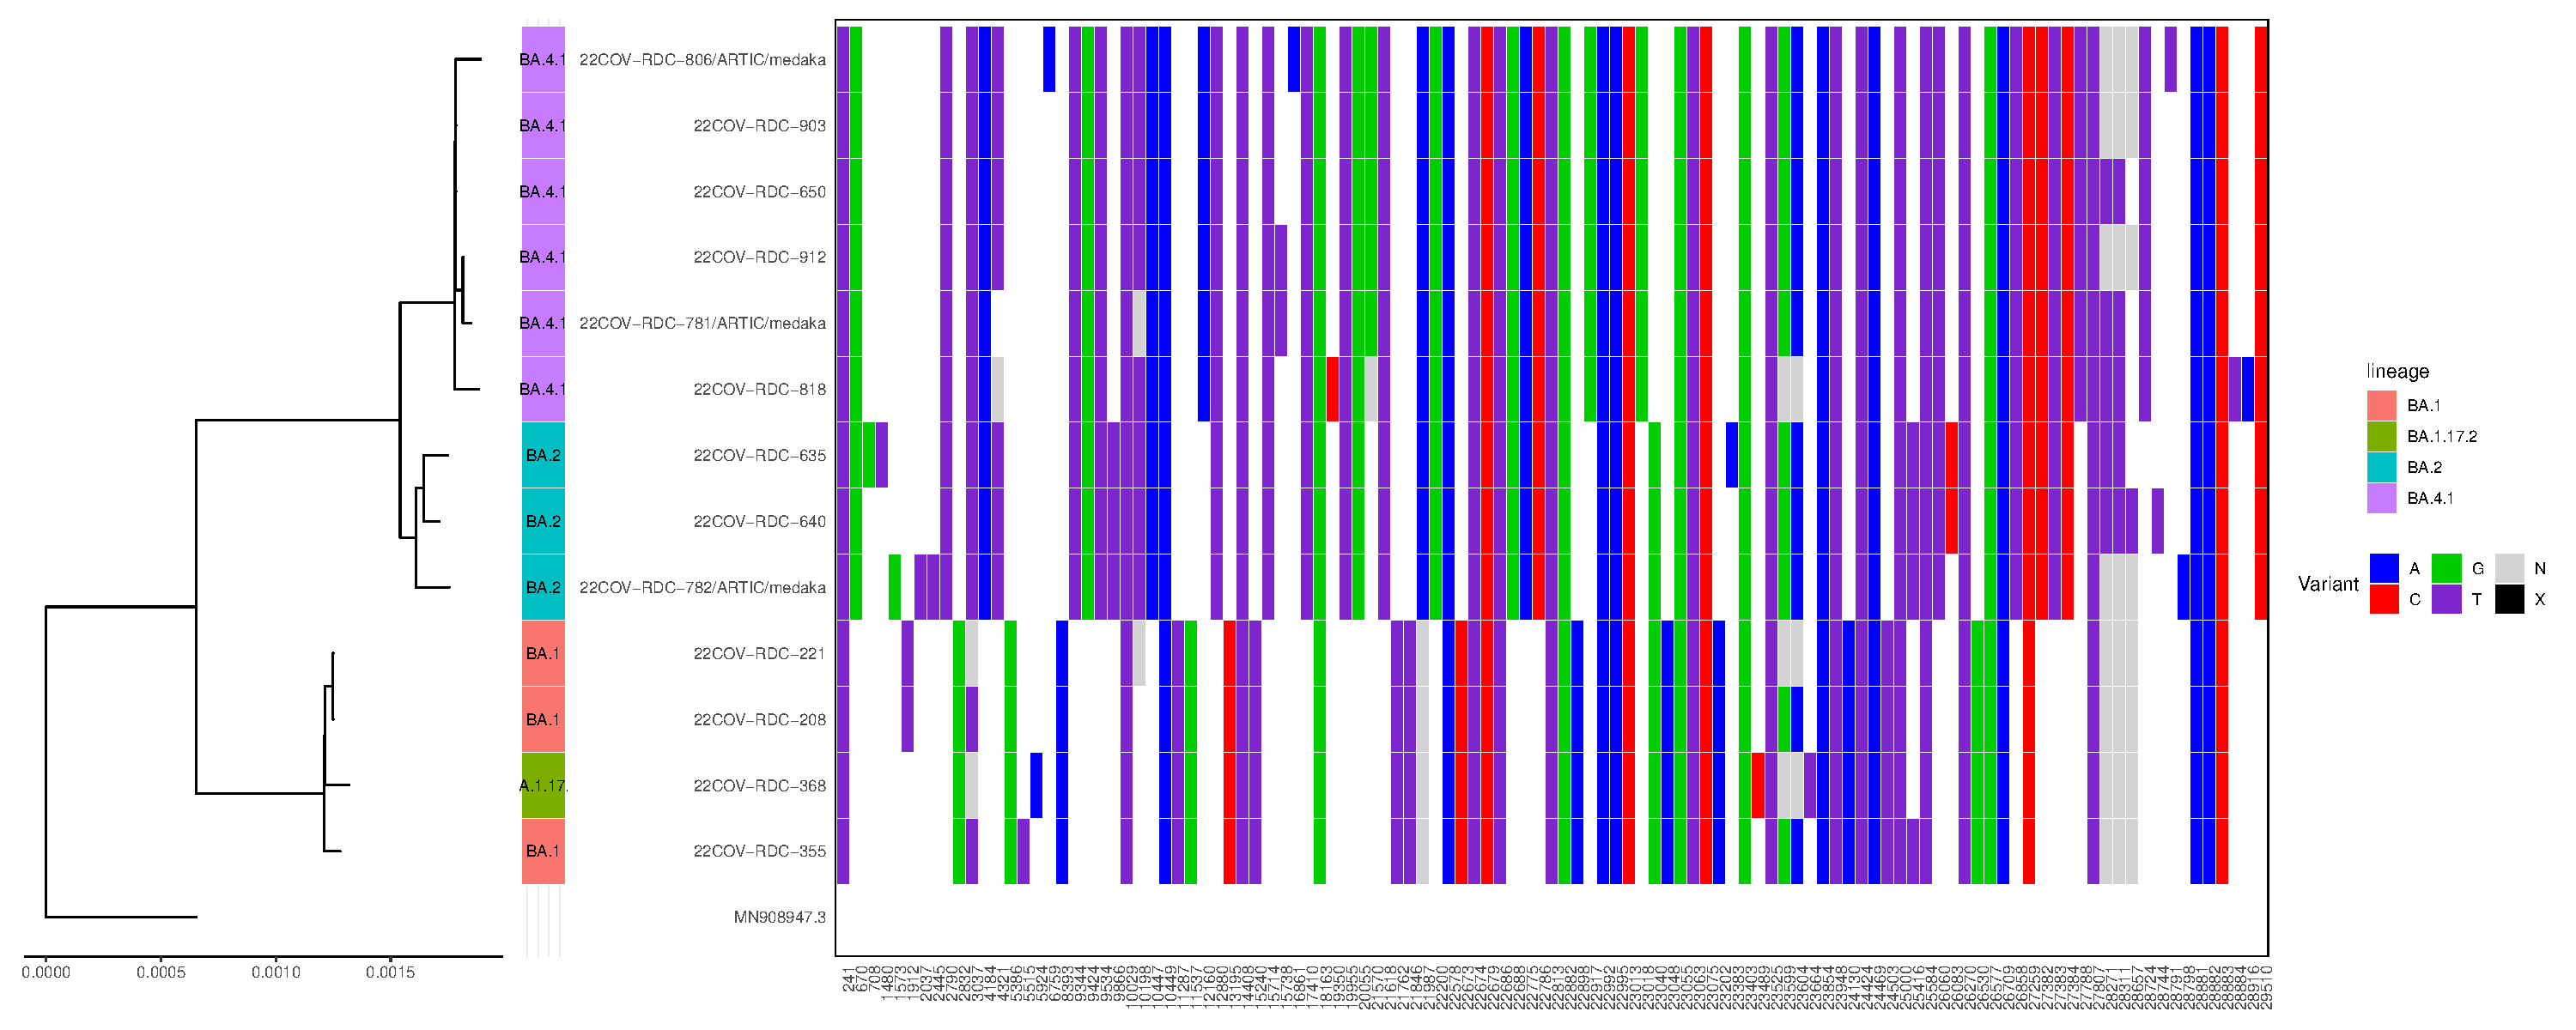
\includegraphics[scale=0.400000]{plots/my_run_tree_snps.pdf}
\end{center}
\subsection{Ambiguity Report}
The ambiguity report is not currently supported for Oxford Nanopore data
\subsection{Mixture Report}
The mixture report is not currently supported for Oxford Nanopore data
\section{Negative Control}
Negative control depth plots not found.
Negative control summary table not found.
\section{Flagged Samples}
This table contains samples assigned to VOC lineage by PANGO or contains a notable mutation.\\
PANGO assignments were made with pangolin 4.1.3, pangolin-data 1.15.1.
\begin{center}
\normalsize
\begin{longtable}{{|c|C{1.5cm}|c|C{3cm}|c|C{5cm}|}}
\hline
Sample & Percent Complete & Lineage & Pangolin Notes & Scorpio Call & Notable Mutations \\ \hline
\endhead
22COV-RDC-208 & 96.6 & BA.1 & alt/ref/amb:53/0/3 & Omicron (BA.1-like) & S:del69-70, S:K417N, S:Q493R, S:N501Y, S:P681H, S:P681H \\ \hline
22COV-RDC-221 & 95.1 & BA.1 & alt/ref/amb:50/0/6 & Omicron (BA.1-like) & S:del69-70, S:K417N, S:Q493R, S:N501Y \\ \hline
22COV-RDC-355 & 96.6 & BA.1 & alt/ref/amb:53/0/3 & Omicron (BA.1-like) & S:del69-70, S:K417N, S:Q493R, S:N501Y, S:P681H, S:P681H \\ \hline
22COV-RDC-368 & 95.5 & BA.1.17.2 & alt/ref/amb:50/0/6 & Omicron (BA.1-like) & S:del69-70, S:K417N, S:Q493R, S:N501Y \\ \hline
22COV-RDC-635 & 96.3 & BA.2 & alt/ref/amb:64/0/0 & Omicron (BA.2-like) & S:G142D, S:K417N, S:Q493R, S:N501Y, S:P681H, S:P681H \\ \hline
22COV-RDC-640 & 98.8 & BA.2 & alt/ref/amb:64/0/0 & Omicron (BA.2-like) & S:G142D, S:K417N, S:Q493R, S:N501Y, S:P681H, S:P681H \\ \hline
22COV-RDC-782 & 93.6 & BA.2 & alt/ref/amb:62/0/2 & Omicron (BA.2-like) & S:G142D, S:K417N, S:Q493R, S:N501Y, S:P681H, S:P681H \\ \hline
22COV-RDC-650 & 97.4 & BA.4.1 & alt/ref/amb:64/0/0 & Omicron (BA.4-like) & S:del69-70, S:G142D, S:K417N, S:L452R, S:N501Y, S:P681H, S:P681H \\ \hline
22COV-RDC-781 & 94.1 & BA.4.1 & alt/ref/amb:62/1/1 & Omicron (BA.4-like) & S:del69-70, S:G142D, S:K417N, S:L452R, S:N501Y, S:P681H, S:P681H \\ \hline
22COV-RDC-806 & 93.5 & BA.4.1 & alt/ref/amb:62/0/2 & Omicron (BA.4-like) & S:del69-70, S:G142D, S:K417N, S:L452R, S:N501Y, S:P681H, S:P681H \\ \hline
22COV-RDC-818 & 94.1 & BA.4.1 & alt/ref/amb:60/0/3 & Omicron (BA.4-like) & S:del69-70, S:G142D, S:K417N, S:L452R, S:N501Y \\ \hline
22COV-RDC-903 & 94.5 & BA.4.1 & alt/ref/amb:62/0/2 & Omicron (BA.4-like) & S:del69-70, S:G142D, S:K417N, S:L452R, S:N501Y, S:P681H, S:P681H \\ \hline
22COV-RDC-912 & 94.8 & BA.4.1 & alt/ref/amb:62/0/2 & Omicron (BA.4-like) & S:del69-70, S:G142D, S:K417N, S:L452R, S:N501Y, S:P681H, S:P681H \\ \hline
\end{longtable}
\normalsize
\end{center}
\section{Sample-level QC}
This table contains QC metrics and warning flags for each sample within this sequencing run.
\begin{center}
\scriptsize
\begin{longtable}{{|c|C{1.3cm}|C{1.3cm}|C{1.0cm}|C{1.0cm}|C{1.0cm}|c|c|C{1.2cm}|C{4.0cm}|}}
\hline
Sample & Consensus SNVs & Consensus IUPAC & Variant SNVs & Variant Indels & Variant Triplet Indels & ct & Date & Percent Complete & QC flags \\ \hline
\endhead
22COV-RDC-208 & 54 & 0 & 49 & 8 & 6 & NA & NA & 96.6 & PASS \\ \hline
22COV-RDC-221 & 51 & 0 & 45 & 8 & 6 & NA & NA & 95.1 & PASS \\ \hline
22COV-RDC-355 & 55 & 0 & 50 & 8 & 6 & NA & NA & 96.6 & PASS \\ \hline
22COV-RDC-368 & 53 & 0 & 47 & 8 & 6 & NA & NA & 95.5 & PASS \\ \hline
22COV-RDC-635 & 71 & 0 & 67 & 6 & 4 & NA & NA & 96.3 & PASS \\ \hline
22COV-RDC-640 & 70 & 0 & 67 & 6 & 3 & NA & NA & 98.8 & PASS \\ \hline
22COV-RDC-650 & 70 & 0 & 66 & 8 & 5 & NA & NA & 97.4 & PASS \\ \hline
22COV-RDC-781 & 69 & 0 & 66 & 8 & 5 & NA & NA & 94.1 & PASS \\ \hline
22COV-RDC-782 & 69 & 0 & 66 & 5 & 2 & NA & NA & 93.6 & PASS \\ \hline
22COV-RDC-806 & 71 & 0 & 67 & 6 & 4 & NA & NA & 93.5 & PASS \\ \hline
22COV-RDC-818 & 69 & 0 & 63 & 8 & 5 & NA & NA & 94.1 & PASS \\ \hline
22COV-RDC-903 & 68 & 0 & 64 & 7 & 4 & NA & NA & 94.5 & PASS \\ \hline
22COV-RDC-912 & 69 & 0 & 65 & 7 & 4 & NA & NA & 94.8 & PASS \\ \hline
\end{longtable}
\normalsize
\end{center}

\end{document}
